\label{sec:uncovering}
There are massive topics related to healthcare and diseases and them expand everyday, it's impractical to list them all. \cite{tuarob2013discovering} defined health-related messages as follows: (1) either a message indicates explicitly the sick (or health problems) of the author; (2) or the message contains the author's worries about health problems (e.g. someone else falling ill, disease outbreak). To surveille diseases, we want to cluster messages(tweets) into different groups, find out what topics are concerned about. The aim of this section is to build a model (or a ensemble of different models) that can: (1) check wether a input document is related to health; (2) assign the checked document to one best match topic. If there is no topic match it, create a new one and assign the document to it (one similar example is hot event discovery). To achieve this, the model should be able to: (1) update the parameters over new input; (2) handle unseen input (such as new words, new topics, new meaning of a seen word, etc.). As far as we know, there is no such model.
\\\\
In the existing works, there are two types of models: supervised and unsupervised. \cite{serban2019real,aramaki2011twitter,lampos2010flu,chen2017disease} use supervised machine learning and deep learning techniques to detect flu. Their experimental results show that when used to detect the known disease, supervised models can get high accuracy. However, the performance of such model highly depends on the training set. For topics that are not in the training set, supervised models cannot recognize it. 
Hence a single end-to-end supervised model (label the data in advance) is not be qualified under this scenario. \cite{paul2012model} introduces Ailment Topic Aspect Model (ATAM) that amis to classify aliments. ATAM is an unsupervised model, requires a set of aliments and the prior distribution of them. Its essence is an variant of LDA, and the hyper-parameter K (the number of diseases/topics) is defined before training. Since the aliments and symptoms are pre-defined, ATAM cannot be treated as a pure unsupervised model, and it can't recognize new health event. However, pure unsupervised models cluster data based on its structure, and therefore are not able to identify whether a document is health-related or not. In addition, the generated topics are hard to interpret. Hence, to achieve the requirements of our model, both supervised and unsupervised methods are required.
\\\\
To extract health-related tweets and topics, \cite{paul2014discovering, paul2011you} described a general framework with 2 main phases: data filtering and topic modeling. The first phase is vital for narrowing down search space. They adopt keyword searching and machine learning as data filtering method. 269 keywords and 20,000 keyphrases were collected and used to filter out irrelevant data roughly. Then 5128 tweets selected randomly from dataset were labeled for training a SVM classifier that identifies wether a input is or isn't health-related. In the second phase, probabilistic topic modeling such as LDA and ATAM are used to cluster tweets and get interpretable topics. \cite{serban2019real,sadilek2012modeling} followed the same framework to classify tweets in their system, with some variance on data labeling, keywords list and classifier. \cite{elkin2017network} used exclusion list rather a classifier in phase one. 
\\\\
Before adopting any existing framework, we used Online Biterm Term Modeling (OBTM, a unsupervised Topic modeling algorithm, details can be found in section \ref{sec:topic modeling}) on a sample of processed data, to see how many health-related topics can be found. The sample covers all processed tweets created at Jan 2018 (13,643,710 non-retweet english tweets). The algorithm took three days on calculation to cluster documents into 100 topics. Merely few topics contain words related to health while they are hard to interpret. Similar experimental results can be found in \cite{zhao2011comparing}, where the authors calculate the distribution of topic categories, and find that roughly 5\% tweets are about health. To narrow down the search space, decrease the running time and make the final results more interpretable, our project adopts a similar framework with \cite{paul2014discovering}: use the keywords search first, then cluster topics. The details and experimental results are in following sections.

\section{Keywords search}
\label{sec:Keywords search}
Influenza is one of the most common diseases and is analyzed most by researchers. For scientific comparison, it was used to test the dataset. \cite{aramaki2011twitter} used a simple word look-up of ``influenza'', which may lose massive valuable data. In inspired by \cite{lamb2013separating,lampos2010flu}, we create a list with 26 words highly related to flu based on Flu Symptoms \cite{cdc.symp} Cambridge Dictionary \cite{cambridge} and relatedwords.org \cite{relatedwords.org}. The complete word list can be seen in table \ref{tab:words list}, note that not all the words from the sources are added to our list. Professional terms are excluded since they are hardly used in colloquialism. Words that are wildly used in other scenarios (such as chill, cold) and phrases that contain keywords in our list (such as asian influenza) are not added. Then tweets are filtered according to the list (ignore case). In this step, we initially adopted a relatively lose filtering strategy: accept tweets containing any string in our list. 
\begin{table}[!htbp]
    \centering
    \hspace{0.5cm}
    \begin{tabular}{p{90pt}p{320pt}}
        Source & Word list \\ \hline
        \href{https://www.cdc.gov/flu/symptoms/symptoms.htm}{CDC} &  fever, feverish, sore throat, runny nose, stuffy nose, headache, nasal congestion, diarrhea, bluish lips, bluish face, dehydration\\ \hline
        \href{https://dictionary.cambridge.org/us/topics/disease-and-illness/colds-and-flu/}{Dictionary} & flu, catarrh, cough, common cold, influenza, sniffle, snuffle\\ \hline
        \href{https://relatedwords.org/relatedto/flu}{relatedwords.org} & h1n1, h5n1, coughing, cholera, ebola, epidemic, feverous, measles \\ \hline
    \end{tabular}
    \caption{Inclusion list}
    \label{tab:words list}
\end{table}
\\
Table \ref{tab:filtering} shows the number of left tweets after keywords filtering with this list. The test sample are tweets posted in the first 5 days of Oct 2018 (with retweets), and in Jan 2018 (without retweets). 
\begin{table}[!htbp]
    \centering
    \hspace{0.5cm}
    \begin{tabular}{ccc}
        Date & Original & Filtered \\ \hline
        2018/10/01 & 4317376 & 5984 \\
        2018/10/02 & 4349129 & 5740 \\
        2018/10/03 & 4417333 & 5415 \\
        2018/10/04 & 4337327 & 5676 \\
        2018/10/05 & 4273031 & 5190 \\
        2018/01 & 134704400 & 37519 \\
    \end{tabular}
    \caption{Tweet counts after flu-related keywords filtering}
    \label{tab:filtering}
\end{table}
\\\\
The result corresponds with experiment conducted by \cite{culotta2010towards}, where the majority of the filtered tweets are irrelevant to keywords. The possible reasons could be that people will use those words even when they are healthy (such as headache), and some words are substring of other words (such as chill-Achill, flu-influence). Another problem found after this step is that the volume of filtered data is far less than expectation. When retweets are included, nearly 0.129\% data are left. Exclude retweets, the percentage drops to 0.0279\% (although the experiment doesn't operate on a same sample set). In the initial design, geo-tagged tweets (tweets with geographic information) created at certain regions are required. According to \cite{sloan}, geo-tagged tweets are scarce (less than 5\% in their experiment), meaning that the percentage of target data could be much lower (less than 0.001\%). Under such condition, massive data are required to get a reliable estimation. To get 10000 filtered data, at least 100000000 metadata are required. The results indicate that, our dataset may be insufficient for analyzing a single disease (such as flu) when the geographic information is required. Therefore, to get a reliable and convincing dataset, we treat all diseases as a whole, expand the inclusion list to more than 9,000 keywords and keyphrases. The sources are given in \cite{paul2011you}. Table \ref{tab:filtering2} shows the filtering results with new keywords list. More than 30 thousand tweets per day are left, which we believe is sufficient for analysis.
\begin{table}[!htbp]
    \centering
    \hspace{0.5cm}
    \begin{tabular}{ccc}
        Date & total & average(per day) \\ \hline
        2018/01 & 3590773 & 115831 \\
        2018/02 & 1087720 & 40285 \\
        2018/03 & 1108867 & 35769 \\
        2018/04 & 769700 & 33465 \\
        2018/10 & 1035587 & 33406 \\
    \end{tabular}
    \caption{Tweet counts after health-related keywords filtering}
    \label{tab:filtering2}
\end{table}

\section{Supervised classification}
\label{sec:Supervised classification}
Keywords search helps to screen out the majority of unrelated data. However, as proved in the experiment, it can't guarantee the purity of the rest. To alleviate the content-irrelevance problem found after first round screening, further filtration is required. \cite{elkin2017network} created another exclusion dictionary containing keywords and phrases indicating tweets should not be included in the filtered dataset, such as "sick and tired". Their experimental result shows such method provides roughly 70\% accuracy on their dataset. This method is easy to implement while its accuracy is highly affected by the choice of exclusion words. In section \ref{sec:unsupervised}, we will use unsupervised method to cluster document. Therefore, the outcome of this step decides the final performance of our model. To get a higer accuracy, we decide to use machine learning based classification methods \cite{aramaki2011twitter}. The model we trained in this step is a binary classifier, aiming to detect health-related tweets. Following are our detailed steps:
\begin{enumerate}
    \item Data classification: Labeling strategies are various for different uses. \cite{lampos2010flu} labeled their data with three categories, positive, negative and unknown. We adopt a simple binary labeling strategy, since the ambiguity will decrease the performance of unsupervised clustering used in the next section. Document will be labeled 1 if it indeed related to health and can easily be recognized, 0 otherwise. One exception is our news dataset, since all the documents were posted by official healthy news channels (such as BBChealth, CDChealth), we treat them all as positive samples (63279 tweets in total with 59902 unique words). Apart from that, we randomly labeled 50000 negative samples based on the keywords list. 20\% data are held out as test set while 20\% of training set are used as validation set at each training epoch.
    \item Word embeddings: This step aims to transform documents into vectors and create a look-up table. There are generally two transforming methods: (1) randomly initialise word vector for each word and then continuously update them by learning; (2) pre-train word embeddings on training set. The former one is easy to implement but will need more time on training and it depends more on training set. In our project, we choose to load word embeddings that was pre-trained on large dataset to save training time and increase accuracy. If a word is in the pre-defined dictionary, we will use its vector directly. Otherwise we will initialise its word vector and train it during training. Word2vec\cite{mikolov2013efficient}, Fasttext\cite{joulin2016bag} and Glove \cite{pennington2014glove} are three most common algorithms used to train word embeddings. Although the theories behind them are different, researchers have proven that there is no significant difference among them in practice. While Fasttext and Word2vec train the word vectors through neural networks that are hard to interpret, Glove adopt a more comprehensive method: getting the word representation based on word co-occurrence. For convenience, we use the pre-trained Glove vectors trained on 2 billion tweets with 27 billion tokens and 1.2 million vocabularies. Each word is represented by a 100-dimension vector \cite{pennington2014glove}. A unique index is assigned to each word and its corresponding vector to form up a look-up table. Each document is then transformed to a 2-D matrix based on the table. Note that the number of vocabularies varies among documents. Text can't be reshaped as images, the common solution is pre-define the maximum length of documents and pad missing value with a certain number. In our dataset, most tweets are 5-15 words long, therefore, we define the maximum length of a document is 15. For tweets having less than three words, they are not included in training set. In our implementation, we handle special terms in following rules: For words that either frequently appear in corpus or merely contained by few documents, they are excluded from the document; (2) string `$<pad>'$ is used to pad missing value to extend sentence, and its vector is initialised with zeros; (3) out of vocabulary (OOV) words in new data are represented by string `$<unk>$'. To get meaningful words referring to an extracted topic, we exclude stop words listed by NLTK (The Natural Language Toolkit) \cite{journals/corr/cs-CL-0205028}.
    \item Evaluation: We choose binary cross entropy loss as the loss function while training the model. The formula is: $$\text{loss}(x, class) = -\log\left(\frac{\exp(x[class])}{\sum_j \exp(x[j])}\right)
    \\                     = -x[class] + \log\left(\sum_j \exp(x[j])\right)$$
    Accuracy and F1 score are used to evaluate the performance of the model, their formulas can be found in section \ref{sec:evaluation}.
    \item Modeling and training: The experiment conducted by \cite{serban2019real} shows that deep neural network (DNN) outperform traditional machine learning models such as SVM. With the Glove word representation technique \cite{pennington2014glove}, their model reaches more than 80\% accuracy on their dataset. Based on that, we adopt DNN based models. A basic NLP DNN includes three parts: embedding layer, hidden layers and output layer. Most state-of-the-art models (such as XLNet \cite{yang2019xlnet}) adopt transfer learning to improve their performance. Since our focus is not the improvement on supervised algorithm, and our dataset is relatively small, we assume that neural network with simple structure can meet our expectation. TextCNN \cite{kim2014convolutional} uses multiple different-size kernels to capture features of documents, with a pooling layer and a fully connected layer. After 20 epochs of training, it gets more than 99\% accuracy on training set and more than 98\% accuracy on both validation set and test set. The accuracy hardly improves after 30 epochs. 
    \item Implementation: the major toolkits used for the implementation of our supervised model are Pytorch and Gensim, source code and trained model can be found in \href{https://github.com/NonBee98/FYP}{our GitHub repository} or in the submitted files.
\end{enumerate}
Table \ref{tab:sup1} shows 11 prediction examples of this model. As mentioned before, the accuracy of this model reaches 98.17\% on our test data and 98.2\% on validation set. The table contains both correct and incorrect predictions. Class 1 represents healthcare-related, 0 otherwise. No.1 to No.6 are correct predictions. However, we mainly care about wrong predictions. Document from No.7 to No.11 are typical incorrect prediction samples. In our training set, word ``canada'' appears more in negative samples, therefore, sentences with ``canada'' are more likely be predicted as positive sample. Word ``booze'' is not in training set, therefore No.8 can't be correctly recognized. No.9, No.10 and No.11 are noises, and the model indeed correctly classifies them. Based on this observation, the accuracy of this model can be improved by: (1) training on more data; (2) exclude frequent word; (3) using more advanced methods to handle out-of-vocabulary problem (such as unknown word inference). 
\begin{table}[!htbp]
    \centering
    \hspace{0.5cm}
    \begin{tabular}{|p{15pt}|p{250pt}|p{60pt}|p{60pt}|}
        \hline
        No. & Text & True class & Prediction \\ \hline
        1 & the move to digital health care is the future but recruitment and training of quality staff needs to happen al & 1 & 1 \\\hline
        2 & catholic school less think kids missed point know literally eve & 0 & 0 \\\hline
        3 & nfl wants players suit over concussions dismissed & 1 & 1\\\hline
        4 & ravaged by typhoon philippines faces threat of serious diseases & 1 & 1 \\\hline
        5 & obama presses leaders to speed ebola response & 1 & 1 \\\hline
        6 & meat seafood prices rising on drought and disease usda & 1 & 1 \\\hline
        7 & wrong initio canada arrest america doesn & 0 & 1 \\\hline
        8 & booze still kills people week & 1 & 0 \\\hline
        9 & top job opportunity ambulance professionals emt nurses physicians around world & 0 & 1 \\\hline
        10 & ad feature & 1 & 0 \\\hline
        11 & course patients first work medical field got stay focused & 0 & 1 \\\hline
    \end{tabular}
    \caption{Sample prediction results of Supervised model}
    \label{tab:sup1}
\end{table}

\section{Unsupervised document clustering and topic generation}
\label{sec:unsupervised}
Supervised models help to screen out documents that are health-related. To detect unseen diseases and healthcare events, we seek solutions on unsupervised algorithm. According to \cite{allahyari2017brief}, Embeddings Based Clustering and Probability Based Topic Modeling are two common methods used to group documents. This section will introduce both and provide some experimental results of applying them on our dataset. Then we will explain how our model are build upon them. The evaluation criterion used in this section is topic coherence. Since the generated topics are hard to interpret, scoring each topic with a exact value by human judgments could be difficult and objective, and it requires massive labour. Topic coherence helps to evaluate the quality of generated topics. Experimental results have proven that it has positive correlation with human judgments. In our experiment, we adopt the framework proposed by \cite{roder2015exploring} to calculate the coherence, higer value means more coherent. Some libraries such as Gensim provide APIs for using it. For convenience, we uses the online service provided by \href{https://palmetto.demos.dice-research.org/}{Palmetto}. The Python interface calling the service can be found in our source code. Each generated topic is evaluated by $C_a$, $C_p$ and their sum together. The test dataset is SearchSnippets, it contains 12,295 documents and 5,547 unique words with 8 different topics (other datasets contain more than 20 topics and therefore are not suitable for comprehensibly comparing the generated topics by human judgments). For comparison, the number of cluster in our experiment is the same with that in the test set. 

\subsection{Embeddings based clustering}
\label{sec:Document vector}
A simple way for solving clustering problems is using traditional clustering methods. The idea behind it is projecting original data into a vector space, grouping documents based on clustering algorithm (such as K-means). The key point is how to project documents. Traditional methods used to represent documents includes one-hot encoding, bag-of-words and TF-IDF. For example, gievn a corpus with two sentences: (1) ``John likes to watch movies. Mary likes movies too.''; (2) ``Mary also likes to watch football games''. There are 10 unique words: `football', `too', `to', `also', `games', `Mary', `John', `movies', `watch', `likes'. Sentence 1 then can be represented as shown in table \ref{tab:bow1}.
\begin{table}[!htbp]
    \centering
    \hspace{0.5cm}
    \begin{tabular}{|c|c|c|c|c|c|c|c|c|c|c|}
        \hline
         & football & too & movies & to & also & games & Mary & John & watch & likes \\ \hline
         One-hot & 0 & 1 & 1 & 1 & 0 & 0 & 1 & 1 & 1 & 1 \\\hline
         BOW & 0 & 1 & 2 & 1 & 0 & 0 & 1 & 1 & 1 & 2 \\\hline
         TFIDF & 0 & 0.11 & 0 & 0 & 0 & 0 & 0 & 0.11 & 0 & 0 \\\hline
    \end{tabular}
    \caption{Example of one-hot, bag-of-word and TF-IDF}
    \label{tab:bow1}
\end{table}
Equation \ref{eq:biterm} shows the formula of TF-IDF. TF means term frequency while IDF is the abbreviation of Inverse Document Frequency. $n_{d,i}$ is the count of word i in document d, $|D|$ is the count of documents, $|\{j: w_i \in D_d\}|$ means the number of documents that contain word i (1 is added in case of there is no document containing $w_i$).
\begin{equation}
    \begin{aligned}
        &TF_{d,i} = \frac{n_{d,i}}{\sum_wn_{d,i}}\\
        &IDF_{i} = \log\frac{|D|}{1 + |\{j: w_i \in D_d\}|} \\
        &TFIDF_{d,i} = TF_{d,i} \cdot IDF_{i}
    \end{aligned} 
    \label{eq:tfidf}
\end{equation}
All of the three traditional methods map words to vectors based on the count of words in the whole corpus and hence has no physical and semantic meaning in a vector space. In addition, the dimensionality of them equals to the number of unique vocabularies in the corpus, hence the vectors projected by them are sparse. Therefore, the distance or cosine among them could contain less or no meaning.
\\\\Word embeddings techniques such as Word2vec \cite{mikolov2013distributed,mikolov2013efficient} introduce some techniques of projecting words into distributed dense word vectors (as mentioned in section \ref{sec:Supervised classification}). Word2vec is an unsupervised machine learning algorithm using neural network, and it can learns relationships between words automatically. Each word is represented by a vector with remarkable linear relationships. One example is: vector(“king”) - vector(“man”) + vector(“woman”) =~ vector(“queen”) \cite{journals/corr/cs-CL-0205028}. Such representation is close to human cognition. Inspired by it, documents, topics are possible to be presented in such way. If words, documents and topics share the same space, then their relationships can be calculated easily. For example, if a document vector is more ``close'' to a topic vector, it is more likely belongs to that topic. Doc2vec \cite{le2014distributed} is a variance of Word2vec, it adds one more document vector as the input for each document. Word vectors are shared in corpus while the document is unique for each document. Once the document vectors are trained, clustering algorithms can be applied on them. Here we experiment this method with a simple K-means cluster. 
After the documents are all grouped, the next step is extracting representive keywords for each topic. We use TF-IDF in our experiment to rank the importance of words. 
\\\\
Table \ref{tab:kmeans1} shows the experimental results of K-means based topic modeling. Consider the distinguishability of document vectors and the curse of dimensionality problem in K-means, the dimension of document vectors is set to 40. The final score of generated topics is negative 1.62. Since the k-means algorithm is unstable, we made another 5 experiments on the same data. The final average coherence is -1.052 with 0.366 standard deviation. This negative value shows that such simple method generally has no guidance. To get better coherence, more advanced method should be used.
\begin{table}[!htbp]
    \centering
    \hspace{0.5cm}
    \begin{tabular}{|p{45pt}|p{210pt}|p{30pt}|p{30pt}|p{30pt}|p{30pt}|}
        \hline
        Topic ID & Top\_words(10) & $C_p$ & $C_a$ & sum\\ \hline
        1 & britannica descartes union magician britannica\_article encyclopaedia\_britannica communism meaning fluid manifesto & -0.372 & 0.112 & -0.260\\\hline
        2 & girl episode movie\_episode piano tiger magician lyric tiger\_wood favorite violin & -0.066 & 0.099 & 0.033\\\hline
        3 & stanford\_edu lecture mit ocw einstein aristotle wolfram maa reasoning opencourseware & -0.473 & 0.120 & -0.354\\\hline
        4 & mozilla cisco microprocessor wireless\_access client\_server mspx zdnet cache ibm sourceforge & -0.421 & 0.086 & -0.335\\\hline
        5 & allposters topix sportsline chron cafepress cbs allposters\_com showtime boxing trailer & -0.713 & 0.067 & -0.646\\\hline
        6 & sewing bull sewing\_machine chicago\_bull speed\_test tiger client\_server ticket fund\_budget tiger\_wood & -0.211 & 0.064 & -0.147\\\hline
        7 & economic\_development cba medicare referee public\_health budget senator union agency internship & -0.329 & 0.215 & -0.114\\\hline
        8 & commodity tax fda budget fund\_budget union economic\_development medicare agency loan & 0.034 & 0.169 & 0.203\\\hline
        & & -2.551 & 0.931 & -1.620\\\hline
    \end{tabular}
    \caption{Experimental results of K-means based clustering}
    \label{tab:kmeans1}
\end{table}

\subsection{Probability based Topic Modeling}
\label{sec:topic modeling}
Topic modeling is a typical tool that is frequently used for discovering abstract topics hidden in documents. It mainly uses techniques of Probability. Early progress includes algorithms such as latent semantic indexing (LSI), Unigram language model and Probabilistic latent semantic analysis (PLSA) \cite{hofmann1999probabilistic, baeza1999modern}. Those algorithms abstract document (d), topic (z) and word (w) from corpus, assume that the generation of a document can be considered as picking a sequence of words from dictionary based on certain probabilistic distribution. Latent Dirichlet Allocation (LDA) \cite{blei2003latent} is a more advanced algorithm under bayesian probability framework. Most of current text modeling algorithms are variants of it. It assumes that: a word is the basic unit of a document, one document could have multiple topics; there are various latent topics that can be characterized by a multinomial distribution over words. The generation of a document can be seen in figure \ref{fig:lda}. It can be explained as following steps: 
\begin{enumerate}
    \item For each document d in corpus D:
    \begin{enumerate}
        \item choose the number of words based on poisson distribution and a prior N
        \item choose the topic distribution {$\theta_d$} of this document based on dirichlet distribution with prior {$\alpha$}
    \end{enumerate}
    \item For each word {$w_w$} in document {$d$}:
    \begin{enumerate}
        \item choose its topic {$z_w$} based on multinomial distribution with prior {$\theta_d$}
        \item choose a word {$w_w$} based on multinomial probability with prior {$z_w$} and {$\beta$}
    \end{enumerate}
\end{enumerate}
\begin{figure}[!htp]
    \centering
    \begin{tikzpicture}
      [
        observed/.style={minimum size=15pt,circle,draw=blue!50,fill=blue!20},
        unobserved/.style={minimum size=15pt,circle,draw},
        hyper/.style={minimum size=1pt,circle,fill=black},
        post/.style={->,>=stealth',semithick},
      ]
  
      \node (w-j) [observed] at (0,0) {$w_w$};
      \node (z-j) [unobserved] at (-1.5,0) {$z_w$};
      \node (z-prior) [unobserved] at (-3,0) {$\theta_d$};
      \node (z-hyper) [label=above:$\alpha$] at (-4.5,0) {};
      \filldraw [black] (-4.5,0) circle (3pt);
      \node (w-hyper) [label=above:$\beta$] at (-1.5,1.5) {};
      \filldraw [black] (-1.5,1.5) circle (3pt);
      
      \path
      (z-j) edge [post] (w-j)
      
      (z-hyper) edge [post] (z-prior)
      (z-prior) edge [post] (z-j)
  
      (w-hyper) edge [post] (w-j)
      ;
  
      \node [draw,fit=(w-j) (z-prior), inner sep=14pt] (plate-context) {};
      \node [above right] at (plate-context.south west) {$D$};
      \node [draw,fit=(w-j) (z-j), inner sep=10pt] (plate-token) {};
      \node [above right] at (plate-token.south west) {$N$};
  
    \end{tikzpicture}
    \caption{Plate Diagram of LDA.\cite{blei2003latent}}
    \label{fig:lda}
  \end{figure}
By training, the word distribution among topics $P(w|z)$ and the topic distribution among documents $P(z|d)$ can be calculated. Then, each document could be assigned to a topic based on its topic distribution. Each topic can be represented by the first few words that are more likely belong to it. 
\begin{table}[!htbp]
    \centering
    \hspace{0.5cm}
    \begin{tabular}{|p{45pt}|p{210pt}|p{30pt}|p{30pt}|p{30pt}|p{30pt}|}
        \hline
        Topic ID & Top\_words(10) & $C_p$ & $C_a$ & sum\\ \hline
        1 & wikipedia football soccer encyclopedia wiki wikipedia\_wiki wikipedia\_encyclopedia basketball rugby world & -0.000 & 0.204 & 0.204\\\hline
        2 & system resource business research information political service gov library web & 0.335 & 0.187 & 0.521\\\hline
        3 & sport news tennis com hockey club yahoo volleyball score gymnastics & 0.334 & 0.247 & 0.581\\\hline
        4 & player health school home information journal college page home\_page union & -0.136 & 0.141 & 0.004\\\hline
        5 & edu science research amazon university book culture theory com amazon\_com & 0.211 & 0.248 & 0.459\\\hline
        6 & game news sport com movie online democracy play video olympic & 0.173 & 0.202 & 0.375\\\hline
        7 & tournament com online art google search golf photo music degree & 0.082 & 0.204 & 0.286\\\hline
        8 & match party computer republic cancer poker gov democratic president presidential & 0.025 & 0.239 & 0.264\\\hline
        & & 1.023 & 1.671 & 2.694\\\hline
    \end{tabular}
    \caption{Experimental results of LDA}
    \label{tab:LDA1}
\end{table}
\\\\Table \ref{tab:LDA1} shows the experimental result of it. We use the Gensim's implementation, parameters of this model is set to default. After 100 iteration's training, the model gets 2.694 score. Topic 3 gets the higest sum coherence, it can be easily classified to sport related topic by human. Since the parameters of LDA is randomly
initialised, each time the output could be different. We made 5 more experiments, and the average sum coherence is 2.64.
\\\\In addition to LDA, we experiment with another more advanced topic model, Biterm Topic Model (BTM) \cite{yan2013biterm, cheng2014btm}, which is designed to modeling short text such as tweets. Figure \ref{fig:btm} demonstrates the generation of corpus in BTM.
\begin{figure}[!htp]
    \centering
    \begin{tikzpicture}
      [
        observed/.style={minimum size=15pt,circle,draw=blue!50,fill=blue!20},
        unobserved/.style={minimum size=15pt,circle,draw},
        hyper/.style={minimum size=1pt,circle,fill=black},
        post/.style={->,>=stealth',semithick},
      ]
  
      \node (w-1) [observed] at (0,0.8) {$w_1$};
      \node (w-2) [observed] at (0,-0.2) {$w_2$};
      \node (z-j) [unobserved] at (-1.5,0) {$z_b$};
      \node (z-prior) [unobserved] at (-3,0) {$\theta$};
      \node (z-hyper) [label=left:$\alpha$] at (-4.5,0) {};
      \filldraw [black] (-4.5,0) circle (3pt);
      \node (w-hyper) [label=right:$\beta$] at (2,0) {};
      \filldraw [black] (2,0) circle (3pt);
      
      \path
      (z-j) edge [post] (w-1)
      (z-j) edge [post] (w-2)
      
      (z-hyper) edge [post] (z-prior)
      (z-prior) edge [post] (z-j)
  
      (w-hyper) edge [post] (w-1)
      (w-hyper) edge [post] (w-2)
      ;
  
      \node [draw,fit=(w-1) (z-j), inner sep=14pt] (plate-context) {};
      \node [above right] at (plate-context.south west) {$B$};
  
    \end{tikzpicture}
    \caption{Plate Diagram of BTM.\cite{yan2013biterm}}
    \label{fig:btm}
\end{figure}
LDA works well on long document such as news, column reports. However, since it captures the word co-occurrence pattern at document-level, its performance may decrease when running on short document such as tweets due to word sparsity problem \cite{yan2013biterm}. BTM provides a feasible solution on short text modeling, it learns the co-occurrence pattern of unordered word pairs (a Biterm) at corpus-level and gets a better retrieval result than LDA and PLSA on short text in the experiment conducted by \cite{yan2013biterm}. The idea behind BTM is that, one words could contain multiple meaning under different scenarios and topics, while a word-pair is more likely belongs to one topic. Documents are then transformed to their corresponding biterms, and the likelihood of the corpus is defined as $P(B|\theta)$ rather than $P(D|\theta)$. 
Table \ref{tab:BTM1} shows the experimental results of BTM applied on SearchSnippets dataset.
\begin{table}[!htbp]
    \centering
    \hspace{0.5cm}
    \begin{tabular}{|p{45pt}|p{210pt}|p{30pt}|p{30pt}|p{30pt}|p{30pt}|}
        \hline
        Topic ID & Top\_words(10) & $C_p$ & $C_a$ & sum\\ \hline
        1 & research edu science information school journal university program gov home & 0.323 & 0.221 & 0.543\\\hline
        2 & movie music com art film video news review photo online & 0.373 & 0.277 & 0.650\\\hline
        3 & wikipedia encyclopedia political system wiki wikipedia\_wiki culture party theory wikipedia\_encyclopedia & 0.064 & 0.167 & 0.231\\\hline
        4 & computer software system web programming memory internet intel com data & 0.249 & 0.223 & 0.472\\\hline
        5 & sport news game football com soccer world match league team & 0.445 & 0.322 & 0.767\\\hline
        6 & business market news stock service trade job finance com information & 0.312 & 0.196 & 0.508\\\hline
        7 & health information cancer disease gov medical drug news calorie healthy & 0.479 & 0.190 & 0.669\\\hline
        8 & amazon com book car amazon\_com engine wheel motor war electrical & -0.034 & 0.190 & 0.156\\\hline
        & & 2.211 & 1.786 & 3.997\\\hline
    \end{tabular}
    \caption{Experimental results of BTM}
    \label{tab:BTM1}
\end{table}
\\\\Compared with LDA, BTM gets better coherence on both $C_p$ and $C_a$, its sum score is about 48\% higer than that of LDA. 5 more experiments shows that the average sum coherence of BTM is about 4.031 with standard deviation 0.213. In addition, we manually compare the generated topics in each experiment, and find that topics generated by topic modeling with higer sum coherence (more than 0.45) will not change significantly in different experiments (a property of Gibbs sampling), while topics generated by clustering method are different in each experiment. 

\subsection{Our model}
\label{sec:modeling}
Experimental results show that traditional clustering methods can't help to generate interpretable topics.
Topic model can find representive words of each topic while grouping documents, it's an ideal solution for our purpose. However, it uses the simple bag of words representation, when handle documents with low frequency words, its interpretability will be affected. To mitigate such problem, an intuitive method is to combine topic model with word embeddings. Lda2vec \cite{moody2016mixing} combines LDA and Word2vec by introducing topic vectors and document vectors. Theoretically, Lda2vec can learn topic, word, document vectors simultaneously while calculating the latent topic distribution, however, in practice we find this model requires massive training time, and the generated topics is hard to understand. Embeded Topic Model (ETM) \cite{dieng2019topic} proposes a novel idea that the word distribution of a topic can be drawn from the Categorical Distribution of the inner production of word embeddings and topic vectors, and it shows how to train the model with back propagation. For our purpose, we need model on short text, hence we take the advantages from both ETM and BTM. The generation of a corpus in our model can be seen as follows, $\alpha$ is the topic matrix with size L $\times$ $|Z|$ (L: lengdith of embedding, $|Z|$: number of topics), $\alpha_k$ denotes the vector of $k_{th}$ topic. $\rho$ denotes the word embeddings matrix with size L $\times$ $|V|$ ($|V|$: the number of words):
\begin{enumerate}
    \item For the whole corpus(mini-batch) B:
    \begin{enumerate}
        \item draw a topic distribution $\theta$ $\sim$ $logistc\_normal(\mu, \sigma)$
        \begin{equation}
            \theta=softmax(\omega); \omega \sim Gussian(\mu, \sigma)
            \label{eq:lognormal}
        \end{equation}
    \end{enumerate} 
    \item For each topic z in topic set Z:
    \begin{enumerate}
        \item draw word distribution $\beta_z$ $\sim$ $softmax(\rho^T\alpha_z)$
    \end{enumerate}
    \item For each biterm b in biterm set B:
    \begin{enumerate}
        \item draw a topic assignment $z_b$ $\sim$ $Cat(\theta)$
        \item draw two words $b_{w_1}$, $b_{w_2}$ $\sim$ $\beta_{z,b}$ ($P(b_{w_i}) = \beta_{z,{b_i}}$)
    \end{enumerate}
\end{enumerate} 
\begin{figure}[!htp]
    \centering
    \begin{tikzpicture}
      [
        observed/.style={minimum size=15pt,circle,draw=blue!50,fill=blue!20},
        unobserved/.style={minimum size=15pt,circle,draw},
        hyper/.style={minimum size=1pt,circle,fill=black},
        post/.style={->,>=stealth',semithick},
      ]
  
      \node (w-1) [observed] at (0,0.8) {$w_1$};
      \node (w-2) [observed] at (0,-0.2) {$w_2$};
      \node (z-j) [unobserved] at (-1.5,0) {$z$};
      \node (z-prior) [unobserved] at (-3,0) {$\theta$};
      \node (z-hyper) [label=left:$softmax(\omega)$] at (-4.5,0) {};
      \filldraw [black] (-4.5,0) circle (3pt);
      \node (b-prior) [unobserved] at (2,0) {$\beta$};
      \node (w-hyper) [label=right:$softmax(\rho^T\alpha)$] at (3.5,0) {};
      \filldraw [black] (3.5,0) circle (3pt);
      
      \path
      (z-j) edge [post] (w-1)
      (z-j) edge [post] (w-2)
      
      (z-hyper) edge [post] (z-prior)
      (z-prior) edge [post] (z-j)
  
      (b-prior) edge [post] (w-1)
      (b-prior) edge [post] (w-2)
      (w-hyper) edge [post] (b-prior)
      ;
  
      \node [draw,fit=(w-1) (z-j), inner sep=14pt] (plate-context) {};
      \node [above right] at (plate-context.south west) {$B$};
      \node [draw,fit=(b-prior) (b-prior), inner sep=14pt] (plate-context) {};
      \node [above right] at (plate-context.south west) {$K$};
  
    \end{tikzpicture}
    \caption{Plate Diagram of Our Model.}
    \label{fig:nbtm}
\end{figure}
Choosing logistc normal instead of Dirichlet function as the topic distribution benefits the further parameters inference (parameters of distribution model can be directly optimized by back propagation). Note that the whole corpus share a same topic distribution,$\mu$ and $\sigma$ are two parameters needed to be learnt. $softmax(\rho^T\alpha_z)$ is a probability vector denotes the probability $P(w|z)$ of each word in the whole corpus. The marginal probability of each biterm under topic matrix $\alpha$ and the likelihood of the whole corpus are defined as follows:
\begin{equation}
    \begin{aligned}
        P(b|\alpha) & = P(b_{w_1}|\alpha)P(b_{w_2}|\alpha)\\
        & = \sum_zP(z)P(b_{w_1}|z,\alpha)P(b_{w_2}|z,\alpha) \\
        & = \int P(\omega)P(b_{w_1}|\omega,\alpha)P(b_{w_2}|z,\alpha) d\omega 
    \end{aligned}
    \label{eq:biterm}
\end{equation}
\begin{equation}
    P(B|\alpha) = \prod_bP(b|\alpha)
    \label{eq:corpus}
\end{equation}
In the model, word embeddings $\rho$ is pre-defined parameters while topic embeddings $\alpha$ is unknown and needed to be trained.
To maximize the likelihood is to maximize equation \ref{eq:marginal}:
\begin{equation}
    \begin{aligned}
        \log P(B|a) & = \sum_{b} \log \sum_zP(z)P(b_{w_1}|z,\alpha)P(b_{w_2}|z,\alpha)\\
        & = \sum_{b}\log \int P(\omega)P(b_{w_1}|\omega,\alpha)P(b_{w_2}|\omega,\alpha)d\omega
    \end{aligned} 
    \label{eq:marginal}
\end{equation}
The conditional probability of words $b_{w_1}$ $b_{w_2}$ in biterm b can be calculated by equation \ref{eq:wbi} (the two words belong to one certain topic):
\begin{equation}
    P(b_{w_1}|\omega,\alpha)P(b_{w_2}|\omega,\alpha) = \theta_z^2\beta_{z,b_{w_1}}\beta_{z,b_{w_2}}
\label{eq:wbi}
\end{equation}
$\theta$ is the topic distribution of the whole corpus, which is generated by the logistc normal in equation \ref{eq:lognormal}. $\beta_z,b_{w_i}$ is calculated by $softmax(\rho^T\alpha_k)$ in step 1.
\\\\
The next question is how to infer the parameters. Equation \ref{eq:marginal} can't be directly optimized since the integral of marginal probability $P(b|\alpha)$ is intractable (EM algorithm cannot be used). In LDA and BTM, Gibbs sampling is used to infer parameters. However, such method requires Dirichlet distribution. Since our model draw words based on the production of $\rho^T\alpha$, same method can't be applied. To infer the parameters, we use Variational inference\cite{wainwright2008graphical} instead. Variational inference helps to create a simpler distribution that could best approach the original intractable distribution. By adopting variational inference, the original statistical inference problem becomes an optimization problem. Our goal now is to find a distribution $Q(\omega; \phi)$ that has the least ``difference'' with original untransformed topic distribution of the mini-batch $P(\omega|B)$. Here $\omega$ is the variational distribution and $\phi$ is the variational parameters of q. Once the $Q(\omega; \phi)$ converges, it can replace the real distribution.
In step 2(a), we assume that the original topic distribution of the corpus is drawn from a Gussian distribution, therefore, q is defined as a Gussian, whose mean and variance is calculated by its parameters. The next step is learning the variational parameters. \cite{kingma2013auto} proposes a method that could automatically learn the variational parameter based on given input (in our model is the biterm set B), the process can be seen as below:
\begin{equation}
    Q(\omega;B;\phi;) \leftarrow Gussian(\mu,\sigma)
\label{eq:var1}
\end{equation}
\begin{equation}
    \mu = f(\phi_{\mu}, B)
\label{eq:var2}
\end{equation}
\begin{equation}
    \sigma = g(\phi_{\sigma}, B)
\label{eq:var3}
\end{equation}
Recall that a biterm is a unordered words pair, and in our model, each word is represented by its embedding. Therefore, in our model, each biterm is defined as the sum of its corresponding words' embeddings (equation \ref{eq:biterm2}), and the whole corpus is represented by the sum of all the biterms. As stated before, the pre-trained word embeddings has semantic and physic meaning (e.g. vec(``phone'') + vec(``apple'') = vec(``iphone'')), such representation uses this good property. Each biterm is assigned with semantic meaning, and this information will be used in parameter inference.
\begin{equation}
    \begin{aligned}
        & b = b_{w_1} + b_{w_2}\\
    \end{aligned}
\label{eq:biterm2}
\end{equation}
Function $f(\phi_{\mu}, B)$ and $g(\phi_{\sigma}, B)$ are two neural networks (there is no special requirements of the networks, they could be simple NNs with one linear layer or with more complex structure). They are called ``encoder'' by \cite{kingma2013auto} since they receive a data (or a batch of data) and output the parameters of its corresponding distribution model (in term of Gussian, the outputs are mean and variance). $\phi_{\mu}$ and $\phi_{\sigma}$ are the parameters of this two neural networks respectively, and they will be updated by back propagation.\\\\
The final step is defining the loss function. Recall that $Q(\omega;B;\phi)$ is the  approximation topic distribution (un-softmaxed) and $P(\omega|B)$ is the posterior probability distribution, $\phi$ is the parameter set of q, we want to minimize their ``difference'' (it's obviously that a simple distribution of $Q(\omega;B;\phi)$ will benefit the inference, which is one reason why we use logistc normal in step 2(a)). The ``difference'' between $P(\omega|B)$ and $Q(\omega;B;\phi)$ is commonly evaluated by the  the Kullback-Leibler (KL) divergence \cite{yang2017understanding}. The KL divergence for variational inference is defined as follows: 
\begin{equation}
    \begin{aligned}
        KL(Q(\omega;B,\phi)||P(\omega|B)) & = \int Q(\omega;B,\phi)\log\frac{Q(\omega;B,\phi)}{P(\omega|B)} d\omega\\
        & = - \int Q(\omega;B,\phi)\log\frac{P(\omega|B)}{Q(\omega;B,\phi)} d\omega\\
        & = - \int Q(\omega;B,\phi)\log\frac{P(\omega, B)}{Q(\omega;B,\phi)P(B)} d\omega\\
        & = - L[Q(\omega;B,\phi)] + \log P(B)\\
    \end{aligned} 
    \label{eq:KL}
\end{equation}
\begin{equation}
    \begin{aligned}
    L[Q(\omega;B,\phi)] & = \int Q(\omega;B,\phi)\log P(\omega, B) d\omega + \int Q(\omega;B,\phi) \log Q(\omega;B,\phi) d\omega\\
    & = \mathbb{E}_q[\log P(B|\omega))] - KL(Q(\omega;B,\phi)||P(\omega))
    \end{aligned} 
    \label{eq:elbo}
\end{equation}
KL divergence can be treated as information loss, it is always $\geq$ 0. When KL divergence equals 0, $Q(\omega;B,\phi)$ and $P(\omega|B)$ are the same distribution. In our model, we want the KL divergence could be as small as possible, and this equals to maximize $L[Q(\omega;B,\phi)]$ (the Evidence Lower Bound, $\mathbb{E}$ is the expectation). The final loss of the mini-batch is then defined as shown in equation \ref{eq:loss}:
\begin{equation}
    \begin{aligned}
        loss(model, B, \rho) & = KL(Q(\omega;B,\phi_B)||P(\omega)) - \sum_{b \in B}\mathbb{E}_q\left[\log P(b|\omega,\alpha)\right] 
    \end{aligned}    
    \label{eq:loss}
\end{equation}
All the variables in equation \ref{eq:loss} can be directly computed. By using the automatic derivation technique, parameters of our model can be updated by back propagation. One problem is that random operation cannot be derived(backpropagated) since it doesn't have gradient. For example, given a variable x,y with arbitrary values, and a variable $z = Gussian(x,y)$, $loss(x,y) = (x-y)^2$, back propagation cannot be applied to the loss function. To solve this problem, make the loss function derivable, we use the reparameterization trick \cite{kingma2013auto}. In terms of the same example, z now equals to $x + Gussian(0,1) * y$. The distribution of z is the same, while the latter one can be backpropagated. To use the trick, we adopt the logistc normal rather than Dirichlet in step step 2(a). Pseudocode of training the model can be seen in algorithm \ref{alg:ebtm}.
\begin{algorithm}[!htbp]
    \caption{Model training}
    \label{alg:ebtm}
    \LinesNumbered 
    \KwIn{$D$: documents set $D=\{d_1,d_2\dots d_n\}$\newline
    $\rho$: pre-trained word embeddings
    }
    \KwOut{$\alpha$: learned topic embeddings\newline
    $\phi$: learned parameter set of Q}
    Pre-process D, build vocabulary and encode documents in D to indexes \\
    Initialise a biterm set $B = \{\}$ \\
    \For{$d \in D$}{
        biterms of $d$ $b_d$ = $extract\_biterm(d)$\\
        $B = B \union b_d$
    }
    Initialise topic embeddings $\alpha$ and variational parameters $\phi$ randomly \\
    \For{$i = 1$ to $max\_iteration$}
    {
        Compute word distribution of all topics: $\beta = softmax(\rho^T\alpha) $\\
        Split $B$ into smaller batches $B_{batches}$\\
        \For{
            $X \in B_{batches}$
        }{
            Compute $\mu$ = $f(\phi_{\mu},B)$\\
            Compute $\sigma$ = $g(\phi_{\sigma},B)$\\
            Draw $\theta$ $\sim$ $logistc\_normal(\phi_{\mu},\phi_{\sigma})$\\
            \For{$biterm$ b $\in X$}{
                Compute $P(b_{w_1}|\theta)P(b_{w_2}|\theta) = (\theta^T)^2(\beta_{.,b_{w_1}}*\beta_{.,b_{w_2}})$
                \label{line:16}
            }
        }
        Compute the loss $l$ based on the loss function \\
        \If{$early\_stop(l)$}{
            stop iteration
        }
        Update parameters $\alpha, \phi$ by back propagation
    }
\end{algorithm}
\\\\The trained model then can be used to infer the topic distribution of documents based on the assumption proposed by \cite{yan2013biterm}:
\begin{equation}
    P(z|d) = \sum_{b\in b_d}P(z|b)P(b|d)
\label{eq:doc1}
\end{equation}
\begin{equation}
    P(z|b) = \frac{P(z)P(b_{w_1}|z)P(b_{w_2}|z)}{\sum_zP(z)P(b_{w_1}|z)P(b_{w_2}|z)}
\label{eq:doc2}
\end{equation}
\begin{equation}
    P(b|d) = \frac{n_d(b)}{\sum_bn_d(b)}
\label{eq:doc3}
\end{equation}
In equation \ref{eq:doc1}, the topic distribution $P(z|b)$ of a document is represented by the expectation of the topic proportions of biterms that are extracted from the document. In equation \ref{eq:doc3}, $n_d(b)$ represents the number of biterm b in document d. Pseudocode in algorithm \ref{alg:infer} explains how this inference works on our model (algorithm \ref{alg:ebtm} and \ref{alg:infer} share the same representation of parameters).
\begin{algorithm}[!htbp]
    \caption{Topic inference}
    \label{alg:infer}
    \LinesNumbered
    \KwIn{$d$: a document (encoded)}
    \KwOut{$P(z|d)$: the topic distribution of d}
    Count the number of each biterm b in document $d$ $n_d(b)$\\
    Compute $\mu$ = $f(\phi_{\mu},B)$\\
    Compute $\sigma$ = $g(\phi_{\sigma},B)$\\ 
    Draw $\theta$ $\sim$ $logistc\_normal(\mu,\sigma)$\\
    \For{b $\in$ $B_d$}
    {
        Compute $P(b|d) = \frac{n_d(b)}{\sum_bn_d(b)}$\\
    }
    \For{topic z $\in$ Z}
    {
        \For{b $\in$ $B_d$
        }{
            Compute $P(z|b)$ = $\theta_{z}\beta_{z,b_{w_1}}\beta_{z,b_{w_2}}$\\
            Compute $temp_b = P(z|b)P(b|d)$
        }
        Compute $P(z|d) = \sum_b temp_b$
    }
\end{algorithm}
\\\\Our model is still under implementation, topic embeddings $\alpha$ and variational parameters $\phi$ are represented by three fully connected layers rather than matrixes to make them trainable. There are several basic hyperparameters in our implementation:
\begin{enumerate}
    \item $|Z|$: the number of topics. Same with BTM, $|Z|$ is predefined and can't be changed.
    \item $|V|$: the number of vocabularies. Vocabularies could be from documents outside the corpus. Larger $|V|$ requires more memory and computation cost while the trained model can infer more documents.
    \item $|L|$: the dimensionality of word embeddings. 
    \item $\rho$: the pre-trained word embeddings. In our model description, each column represents a word embedding, however, for the convenience, in our implementation, $\rho$ is transposed ($\rho^T$, with size $|V|\times|L|$). The embeddings can be trained by any algorithms (such as Word2vec, Glove). 
    \item Hidden size: in our implementation, $f(b,\phi)$ and $g(b,\phi)$ are two fully connected layers whose input size is hidden size and output size is $|Z|$. It decides the number of parameters of $\phi$ to be learned.
    \item Activation function: function that adds nonlinearity to $f(b,\phi)$ and $g(b,\phi)$.
    \item Batch size: the number of samples fed to the model each time
\end{enumerate}
\begin{table}[!htbp]
    \centering
    \hspace{0.5cm}
    \begin{tabular}{|p{45pt}|p{210pt}|p{30pt}|p{30pt}|p{30pt}|p{30pt}|}
        \hline
        Topic ID & Top\_words(10) & $C_p$ & $C_a$ & sum\\ \hline
        1 & digital issue service online resource disease medical comprehensive payment center & 0.238 & 0.188 & 0.426\\\hline
    2 & university library edu comprehensive chicago wiki britannica school study center & 0.260 & 0.188 & 0.448\\\hline
    3 & modern publication center journal theoretical study society edu graduate evolutionary & 0.292 & 0.186 & 0.478\\\hline
    4 & information news online com home page research index edu world & 0.247 & 0.202 & 0.449\\\hline
    5 & international information library instruction professional definition link marketing community research & -0.037 & 0.139 & 0.102\\\hline
    6 & geographic grant writing nasa gov link volleyball page reliable history & -0.028 & 0.197 & 0.168\\\hline
    7 & university graduate resource society directory health undergraduate academic center student & 0.472 & 0.239 & 0.711\\\hline
    8 & project data graduation event interview congress topic issue expert conflict & 0.150 & 0.116 & 0.266\\\hline
    & & 1.594 & 1.455 & 3.049\\\hline
    \end{tabular}
    \caption{Experimental results of our model}
    \label{tab:EBTM1}
\end{table}
Table \ref{tab:EBTM1} shows the experimental results of our model on SearchSnippets dataset. The word embeddings is trained on the dataset itself through Word2vec with 300 dimension and 200 iteration. Hidden size is set to 800, and ``tanh'' is used as the activation function. The model gets an average 3.103 sum score in 6 round experiments. By analyzing the results, we can found that certain words have higher probability $P(w|z)$ in all topics, and most of the documents are inclined to one topic, leading the similarity among generated topics. For instance, in this table, topic 7 get the higest sum coherence, and it's obviously that this topic is about education, student. However, topic 2 and 3 can also be regarded as education-related, and they share some same words with topic 7. This observation is proven by tracing back the topic distribution $\theta$: more than 99.99\% documents in the whole corpus belongs to one topic. 
This dataset contains 8 different topics, therefore we want to increase the diversity of generated topics. The improvement is planed to be done in our future work.


\section{Integration and visualization}
Since our model is still under experiment, the final integration is chosen as an ensemble of our trained TextCNN model and BTM. The whole process is wrapped into 4 separate Python scripts: preparedata.py, training.py, filtering.py and clustering.py. To see the demo, directly run the last one (to test our model, run with additional command ``\verb|--|model ebtm''). According to the observation in experiments, we split the generated topics into three rudimentary categories based on their ambiguity:
\begin{enumerate}
    \item clear topics: topics whose first 10 words (sorted by $P(w|z)$) are highly correlated with each other and their implication can be easily understood by human judgments 
    \item ambiguous topics: most of whose first 10 words are in one scope while the rest could be from other scopes (such as word ``health'' appears with ``university  graduate  resource  society  directory   undergraduate  academic center student``'). Exclude such words, the topic could be easily understood.
    \item noise: topics whose first 10 words come from several different scopes and cannot interpret.
\end{enumerate}
In terms of the coherence, based on the experimental results and our own judgments, we make a standard that if the sum coherence of a topic is lower than 0.3, the topic is a noise. Roughly when its sum coherence reaches 0.6, the topic can be regarded as clear. Note that the coherence calculation requires an additional corpus as its reference. As mentioned before, in our experiments, the coherence is computed with the help of Palmetto's online service, whose reference is a collection of english Wikis. When use different reference, the standards will change. In our implementation, we exclude all noisy topics, the remains are visualized by following ways:
\begin{enumerate}
    \item Word cloud: word cloud is commonly used in text visualization tasks, it can help to identify the key information directly and clearly. The font of a word in a word cloud is decided by its ``weight'', bigger font means the word is more important in the corpus. For each topic, we generate a unique word cloud based on its responding $P(w|z)$.
    \begin{figure}[!htbp]
        \centering
        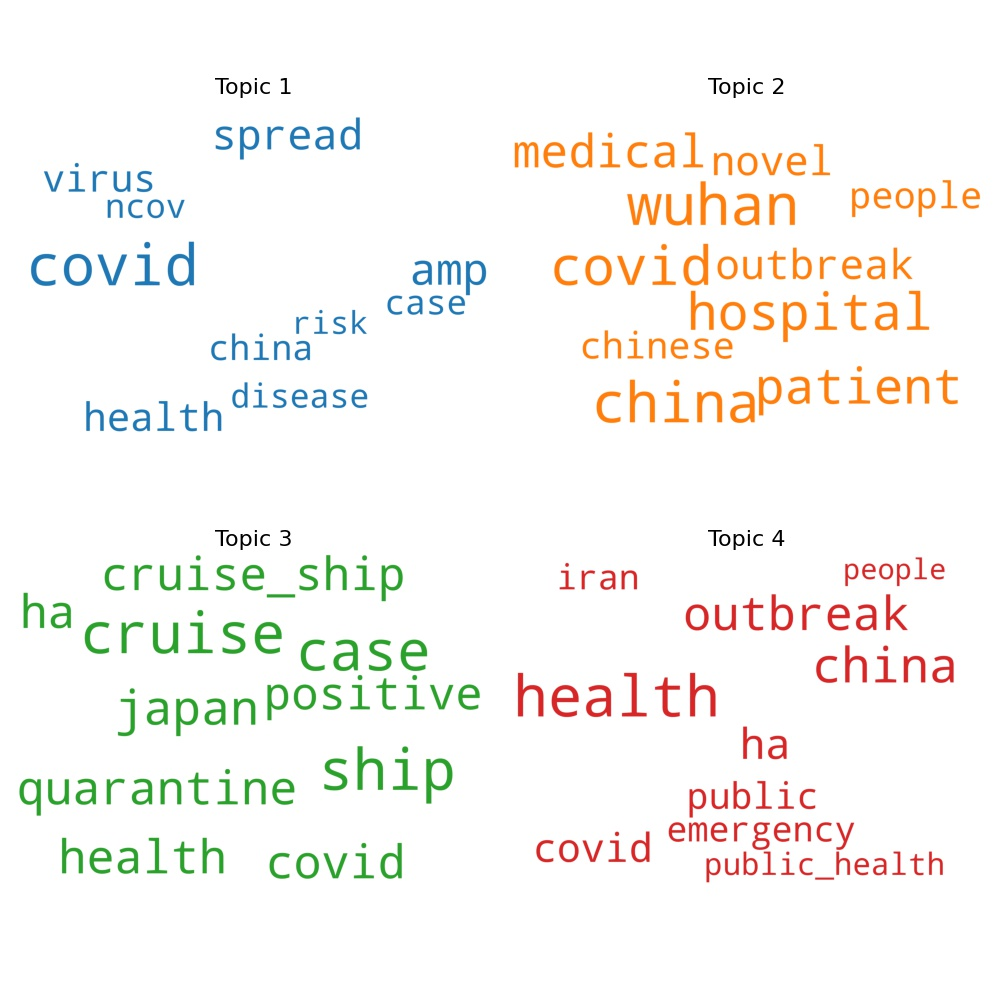
\includegraphics[width=3.5in]{healthnews_word_cloud.jpg}
        \caption{Example of Word Clouds}
        \label{fig:wordcloud}
    \end{figure}
    \\Figure \ref{fig:wordcloud} shows an example of word cloud generated from the our COVID-19 dataset with BTM. For each topic, its key words can be found easily.
    \item Bar chart: word cloud doesn't contain statistical information while bar chart can directly show the trend. For our purpose, we want to know what are the most discussed topics in the corpus, and there are two responding data containing such information: (1) the theoretical topic distribution $theta$; (2) the real topic distribution after assigning the document to the topic that has the highest $P(z|d)$ in that document.
    \begin{figure}[!htbp]
        \centering
        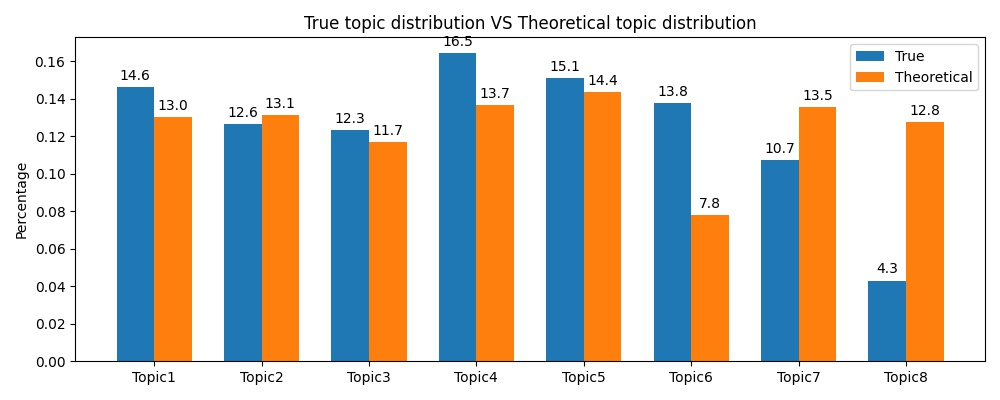
\includegraphics[width=5in]{healthnews_distribution.jpg}
        \caption{Example of Bar chart}
        \label{fig:barchart}
    \end{figure}
    \\Figure \ref{fig:barchart} shows an example of the bar chart, blue bars represents the true distribution while the orange bars represents the theoretical distribution.
\end{enumerate}